\documentclass[tcc,capa]{texufpel}

\usepackage[utf8]{inputenc} % acentuacao
\usepackage{amsmath} % para equações
\usepackage{graphicx} % para inserir figuras
\usepackage[T1]{fontenc}
\usepackage{booktabs} % Para tabelas estéticas
\usepackage{float}    % Para posicionamento de figuras/tabelas
\usepackage{url}      % Para links nas referências


\newcommand{\source}[1]{\par {\small Fonte: #1}}

\hypersetup{
    hidelinks, % Remove coloração e caixas
    unicode=true,   %Permite acentuação no bookmark
    linktoc=all %Habilita link no nome e página do sumário
}

% -------------------------------------------------------------------------
% DADOS DO TRABALHO
% -------------------------------------------------------------------------
\unidade{Centro de Desenvolvimento Tecnológico}
\curso{Engenharia de Computação}
\nomecurso{Bacharelado em Engenharia de Computação}
\titulocurso{Bacharel em Engenharia de Computação}

\unidadeeng{Technology Development Center}
\cursoeng{Computer Engineering}

\title{Plataforma Híbrida de Instrumentação para Biosinais: Redução de Ruído com Hardware de Precisão e Inteligência Artificial}

\author{Menezes}{Gerson Leite de}
\advisor[Prof.~Dr.]{Rossetto}{Alan Carlos Junior}

% Palavras-chave em PT_BR
\keyword{instrumentação biomédica;}
\keyword{processamento de sinais;}
\keyword{inteligência artificial;}
\keyword{hardware de precisão.}

% Palavras-chave em EN_US
\keywordeng{biomedical instrumentation;}
\keywordeng{signal processing;}
\keywordeng{artificial intelligence;}
\keywordeng{precision hardware.}

\begin{document}

% Gera a capa e folha de rosto conforme o estilo texufpel
\maketitle 

\sloppy

% Ficha catalográfica (ajustar conforme biblioteca)
\fichacatalografica

% Folha de aprovação
\begin{aprovacao}{30 de Julho de 2026} 
\noindent Prof. Dr. Alan Carlos Junior Rossetto (orientador)\\
Doutor em Ciência da Computação pela UFRGS.\\[1cm]

\noindent Prof. Dr. Membro da Banca 1\\
Doutor em ... pela ...\\[1cm]

\noindent Prof. Dr. Membro da Banca 2\\
Doutor em ... pela ...\\[1cm]
\end{aprovacao}

% Dedicatória
\begin{dedicatoria}
  Dedico este trabalho aos meus pais e à minha namorada Gessyca, pelo apoio constante e incentivo durante toda a minha jornada acadêmica.
\end{dedicatoria}

% Agradecimentos
\begin{agradecimentos}
  Agradeço aos meus familiares e amigos, que sempre estiveram ao meu lado.
  Ao meu orientador, Prof. Alan Rossetto, pela oportunidade e confiança.
\end{agradecimentos}

% Epígrafe
\begin{epigrafe}
  ``A simplicidade é o grau máximo de sofisticação.''\\
  {\sc --- Leonardo da Vinci}
\end{epigrafe}

% -------------------------------------------------------------------------
% RESUMO
% -------------------------------------------------------------------------
\begin{abstract}
A aquisição de biosinais, como o Eletrocardiograma (ECG) e a Eletromiografia (EMG), é fundamental na saúde e pesquisa, mas estes sinais de baixa amplitude são suscetíveis a ruídos da rede elétrica e artefatos de movimento. Equipamentos profissionais de alta fidelidade possuem custo elevado, enquanto soluções de baixo custo carecem de precisão. Este trabalho propõe o desenvolvimento de uma plataforma híbrida de instrumentação para a aquisição e análise de biosinais, combinando um hardware de alta precisão com pós-processamento via software inteligente. A abordagem se baseia em duas frentes de atuação: primeiramente, o projeto de um \textit{shield} de condicionamento analógico de baixo ruído, responsável por amplificar e filtrar o sinal na sua origem. Em seguida, os dados adquiridos são processados em um computador por um algoritmo de Inteligência Artificial, que atua como uma segunda camada de filtragem adaptativa para atenuar ruídos complexos. Como principal contribuição, espera-se obter uma plataforma funcional de baixo custo que demonstre uma melhora significativa na relação sinal-ruído, validada através da aquisição de sinais reais de ECG e EMG.
\end{abstract}

% -------------------------------------------------------------------------
% ABSTRACT (INGLÊS)
% -------------------------------------------------------------------------
\begin{englishabstract}{Hybrid Instrumentation Platform for Biosignals: Noise Reduction with Precision Hardware and Artificial Intelligence}
The acquisition of biosignals, such as Electrocardiogram (ECG) and Electromyography (EMG), is fundamental in health and research, but these low-amplitude signals are susceptible to power line noise and motion artifacts. High-fidelity professional equipment is expensive, while low-cost solutions lack precision. This work proposes the development of a hybrid instrumentation platform for the acquisition and analysis of biosignals, combining high-precision hardware with intelligent software post-processing. The approach is based on two fronts: firstly, the design of a low-noise analog conditioning shield, responsible for amplifying and filtering the signal at its source. Next, the acquired data is processed on a computer by an Artificial Intelligence algorithm, acting as a second layer of adaptive filtering to attenuate complex noises. As a main contribution, a functional low-cost platform demonstrating a significant improvement in the signal-to-noise ratio is expected, validated through the acquisition of real ECG and EMG signals.
\end{englishabstract}

% Listas de Figuras e Tabelas
\listoffigures
\listoftables

% Lista de Abreviaturas
\begin{listofabbrv}{CMRR} % O parâmetro {CMRR} é a maior sigla para alinhar
    \item[ADC] Analog-to-Digital Converter
    \item[CMRR] Common-Mode Rejection Ratio
    \item[CNN] Convolutional Neural Network
    \item[DAE] Denoising Autoencoder
    \item[DAQ] Data Acquisition
    \item[ECG] Eletrocardiograma
    \item[EMG] Eletromiografia
    \item[ML] Machine Learning
    \item[IA] Inteligência Artificial
    \item[INA] Instrumentation Amplifier
    \item[PCB] Printed Circuit Board
    \item[RNAs] Redes Neurais Artificiais
    \item[sEMG] Surface Electromyography
    \item[SNR] Signal-to-Noise Ratio
    \item[SoC] System on Chip
\end{listofabbrv}

% Sumário
\tableofcontents

% -------------------------------------------------------------------------
% CAPÍTULO 1: INTRODUÇÃO
% -------------------------------------------------------------------------
\chapter{Introdução}

A instrumentação biomédica dedica-se ao desenvolvimento de sistemas para medir e monitorar sinais fisiológicos. Dentre estes, os biopotenciais --- sinais elétricos gerados por atividade celular, como o Eletrocardiograma (ECG) e a Eletromiografia (EMG) --- são dos mais estudados e clinicamente relevantes. Historicamente, a aquisição destes sinais era restrita a ambientes clínicos controlados, utilizando equipamentos analógicos volumosos e de alto custo \cite{goldberger2000}.

Com o avanço da microeletrônica, tornou-se viável o desenvolvimento de sistemas de aquisição de dados (DAQ) portáteis e de baixo custo, frequentemente baseados em microcontroladores. Plataformas como o Arduino popularizaram o acesso a essas tecnologias. No entanto, a aquisição de biosinais apresenta um desafio de engenharia significativo: os sinais de interesse possuem amplitude muito baixa (na faixa de microvolts a milivolts) e seu espectro de frequência se sobrepõe a diversas fontes de ruído, notadamente o ruído da rede elétrica (60 Hz e seus harmônicos) e artefatos de movimento \cite{pathak2025}.

Soluções convencionais de baixo custo frequentemente falham em mitigar esse ruído de forma eficaz. O conversor Analógico-Digital (ADC) nativo de microcontroladores como o ATmega328 (do Arduino Uno) possui resolução e linearidade insuficientes, e o projeto de circuitos de condicionamento analógico --- a etapa de amplificação e filtragem que antecede a digitalização --- é crítico. Um projeto inadequado de \textit{front-end} analógico pode contaminar irremediavelmente o sinal antes mesmo que ele seja processado digitalmente \cite{kim2016}.

Por outro lado, o processamento digital de sinais e, mais recentemente, a Inteligência Artificial, trouxeram novas ferramentas para o tratamento de sinais ruidosos. Contudo, para ruídos complexos e não-estacionários, métodos de filtragem adaptativa \cite{widrow1975} e algoritmos baseados em aprendizado de máquina demonstram superioridade. Redes neurais, como as convolucionais (CNNs) e autoencoders, têm mostrado resultados promissores na reconstrução e remoção de ruído de sinais de ECG \cite{antczak2018}.

Este trabalho se justifica pela lacuna existente entre os sistemas de instrumentação de baixo custo e a necessidade de alta fidelidade na aquisição de biosinais. A inovação do projeto reside na abordagem híbrida: em vez de depender unicamente do hardware ou do software, propõe-se uma sinergia entre ambos. O projeto se distingue de outros por não tentar corrigir um sinal de baixa qualidade (adquirido por hardware genérico) apenas com software. A hipótese é que, ao projetar um hardware de precisão dedicado (um \textit{shield} analógico de baixo ruído), o sinal entregue ao processador será de qualidade muito superior, permitindo que a camada de Inteligência Artificial atue de forma mais fina e eficaz.

\section{Objetivos}

\subsection{Objetivo Geral}
Desenvolver e validar uma plataforma híbrida de instrumentação para aquisição de biosinais (ECG e EMG), que utilize a sinergia entre um \textit{shield} de condicionamento analógico de precisão e algoritmos de Inteligência Artificial para maximizar a relação sinal-ruído.

\subsection{Objetivos Específicos}
\begin{itemize}
    \item Realizar um estudo aprofundado sobre a natureza dos biosinais, técnicas de condicionamento analógico e métodos de IA;
    \item Projetar e simular um circuito de \textit{front-end} analógico de baixo ruído, contendo amplificação de instrumentação e filtragem ativa;
    \item Implementar e validar o protótipo de hardware do \textit{shield}, primeiro em protoboard e, subsequentemente, em placa de circuito impresso (PCB);
    \item Desenvolver o software base de aquisição (firmware) e uma interface de visualização em tempo real;
    \item Implementar e treinar um modelo de Inteligência Artificial para a filtragem adaptativa de ruído;
    \item Integrar o hardware e o software em uma plataforma funcional;
    \item Validar o sistema completo através da aquisição de sinais reais, comparando quantitativamente a relação sinal-ruído.
\end{itemize}

% -------------------------------------------------------------------------
% CAPÍTULO 2: FUNDAMENTAÇÃO TEÓRICA
% -------------------------------------------------------------------------
\chapter{Aquisição e Processamento de Biosinais}

Este capítulo estabelece as bases conceituais necessárias para a compreensão da plataforma desenvolvida. Inicialmente, são apresentadas as características fisiológicas dos sinais biológicos de interesse. Em seguida, discutem-se os princípios de instrumentação biomédica, detalhando os estágios de hardware para condicionamento de sinais. Por fim, abordam-se as técnicas de processamento digital e os fundamentos de Inteligência Artificial aplicados à filtragem e análise de séries temporais.

\section{Biosinais}

Os biosinais são manifestações energéticas mensuráveis que refletem processos biológicos e o estado de funcionamento de sistemas fisiológicos. Eles podem apresentar natureza química, mecânica, térmica ou elétrica, variando no tempo de forma determinística ou estocástica. Na prática clínica e na pesquisa, a análise dessas grandezas é a principal ferramenta para o diagnóstico de patologias e o monitoramento da homeostase corporal, exigindo transdutores específicos para converter essas variações biológicas em sinais elétricos interpretáveis por sistemas de instrumentação \cite{carr2001}.

No contexto da engenharia biomédica, o foco recai predominantemente sobre os biopotenciais: sinais elétricos gerados pela atividade eletroquímica de células excitáveis, como neurônios e fibras musculares. A origem desses sinais reside na dinâmica da membrana celular, onde o fluxo de íons (principalmente sódio, potássio e cálcio) gera potenciais de ação que se propagam através dos tecidos. Quando somados espacialmente e temporalmente, esses microeventos celulares resultam em campos elétricos macroscópicos que podem ser captados na superfície corporal, dando origem a registros clássicos como o Eletrocardiograma (ECG) e a Eletromiografia (EMG) \cite{marchetti2006}.

Contudo, a aquisição desses sinais impõe desafios significativos. Como são captados na superfície da pele através de eletrodos (método não invasivo), os biopotenciais sofrem forte atenuação pelos tecidos biológicos, apresentando amplitudes na ordem de microvolts ($\mu V$) a milivolts ($mV$). Além da baixa amplitude, esses sinais ocupam uma faixa de frequência que frequentemente se sobrepõe a ruídos ambientais e artefatos de movimento, exigindo técnicas rigorosas de amplificação e filtragem para garantir a fidelidade da informação \cite{balbinot2019v1}.

\subsection{Eletrocardiograma (ECG)}
O Eletrocardiograma (ECG) é o registro gráfico da atividade elétrica do coração, captado por eletrodos posicionados na superfície corporal. Ele representa a soma espacial e temporal dos potenciais de ação das fibras miocárdicas durante o ciclo cardíaco. A análise morfológica do ECG é fundamental para o diagnóstico de diversas patologias, como arritmias, isquemias e infartos.

Segundo \cite{souto2016}, um ciclo cardíaco normal em um traçado de ECG é composto por uma sequência de deflexões características, denominadas ondas P, Q, R, S e T. A Onda P representa a despolarização atrial, ou seja, a ativação elétrica dos átrios que antecede a sua contração mecânica. É tipicamente uma onda arredondada e de pequena amplitude (0,1 a 0,2 mV). O Complexo QRS corresponde à despolarização ventricular. É a estrutura mais proeminente do ECG, caracterizada por uma deflexão rápida e de grande amplitude (até 1-2 mV), refletindo a grande massa muscular dos ventrículos. A Onda T representa a repolarização ventricular, momento em que o miocárdio recupera seu potencial de repouso para o próximo batimento.

\begin{figure}[htbp]
    \centering
    \includegraphics[width=0.8\textwidth]{imagens/ecg_padrao.jpg}
    \caption{Sinal de ECG típico mostrando as ondas P, QRS e T.}
    \label{fig:ecg}
\end{figure}

A padronização do registro de ECG é essencial para a análise clínica. O sinal é tradicionalmente impresso sobre uma grade milimetrada padrão, onde cada eixo possui um significado físico preciso. O eixo horizontal representa o tempo: a velocidade padrão de registro é de 25 mm/s. Assim, cada subdivisão menor (1 mm) corresponde a 0,04 segundos (40 ms), e cada quadrado maior (5 mm, composto por 5 quadradinhos) corresponde a 0,20 segundos (200 ms). O eixo vertical representa a voltagem (amplitude): a calibração padrão é de 10 mm/mV. Portanto, cada subdivisão menor (1 mm) na vertical representa 0,1 milivolts (0,1 mV), e cada quadrado maior (5 mm) representa 0,5 mV. Essa padronização permite que médicos e sistemas automatizados calculem a frequência cardíaca e a duração de intervalos críticos (como o intervalo PR e o segmento ST) visualmente.

A análise clínica do ECG baseia-se não apenas na presença das ondas, mas na duração e amplitude dos intervalos entre elas. Segundo \cite{souto2016} e ilustrado na Figura \ref{fig:ecg}, a atividade elétrica cardíaca normal segue um padrão hierárquico e temporal rigoroso:

\begin{itemize}
    \item \textbf{Onda P:} A primeira deflexão do ciclo, correspondente à despolarização atrial. Sua duração normal é inferior a 0,10 s e sua voltagem não deve exceder 0,25 mV. Alterações nesta onda podem indicar sobrecarga atrial.
    
    \item \textbf{Intervalo PR:} Compreende o tempo desde o início da onda P até o início do complexo QRS. Representa o retardo fisiológico da condução elétrica no nó atrioventricular, essencial para permitir o enchimento ventricular antes da contração. Sua duração normal varia entre 0,12 s e 0,20 s.
    
    \item \textbf{Complexo QRS:} Representa a despolarização ventricular. É composto por três ondas: a onda Q (primeira deflexão negativa), a onda R (primeira deflexão positiva) e a onda S (deflexão negativa após a onda R). A duração normal do complexo é de 0,06 s a 0,10 s. Um alargamento deste complexo geralmente indica bloqueios de ramo ou condução ventricular aberrante \cite{souto2016}.
    
    \item \textbf{Segmento ST e Onda T:} O segmento ST reflete o período refratário absoluto dos ventrículos (início da repolarização), devendo estar nivelado com a linha de base (isoelétrico). A onda T representa a repolarização ventricular propriamente dita.
\end{itemize}

A correta identificação destas estruturas no sinal ruidoso é o principal desafio dos sistemas de monitoramento automático, visto que artefatos de movimento (comuns na EMG) podem mimetizar a alta frequência do complexo QRS ou distorcer a linha de base do segmento ST.


\subsection{Eletromiografia (EMG)}
A eletromiografia (EMG) é uma técnica utilizada para o monitoramento da atividade elétrica das membranas excitáveis das células musculares. O sinal eletromiográfico representa a soma algébrica dos potenciais de ação das fibras musculares ativas detectados em uma determinada área \cite{marchetti2006}. Essa técnica é amplamente utilizada tanto em análises clínicas, como no estudo da marcha, quanto em aplicações de controle biomédico, pois fornece informações sobre o tempo de ativação e a intensidade da contração muscular.

Para a aquisição do sinal, comumente utilizam-se eletrodos de superfície (sEMG), que são dispositivos não invasivos aderidos à pele. A interface eletrodo-pele atua como um transdutor que capta a corrente iônica gerada nos músculos e a converte em corrente eletrônica para o sistema de instrumentação. Segundo \cite{marchetti2006}, a configuração bipolar é a mais adequada para esse tipo de aplicação. Nela, dois eletrodos de detecção são posicionados sobre o ventre muscular e um terceiro eletrodo (referência) é colocado em uma região eletricamente neutra. Essa configuração permite o uso de amplificação diferencial, fundamental para eliminar ruídos de modo comum que afetam ambos os eletrodos de detecção.

\begin{figure}[htbp]
    \centering
    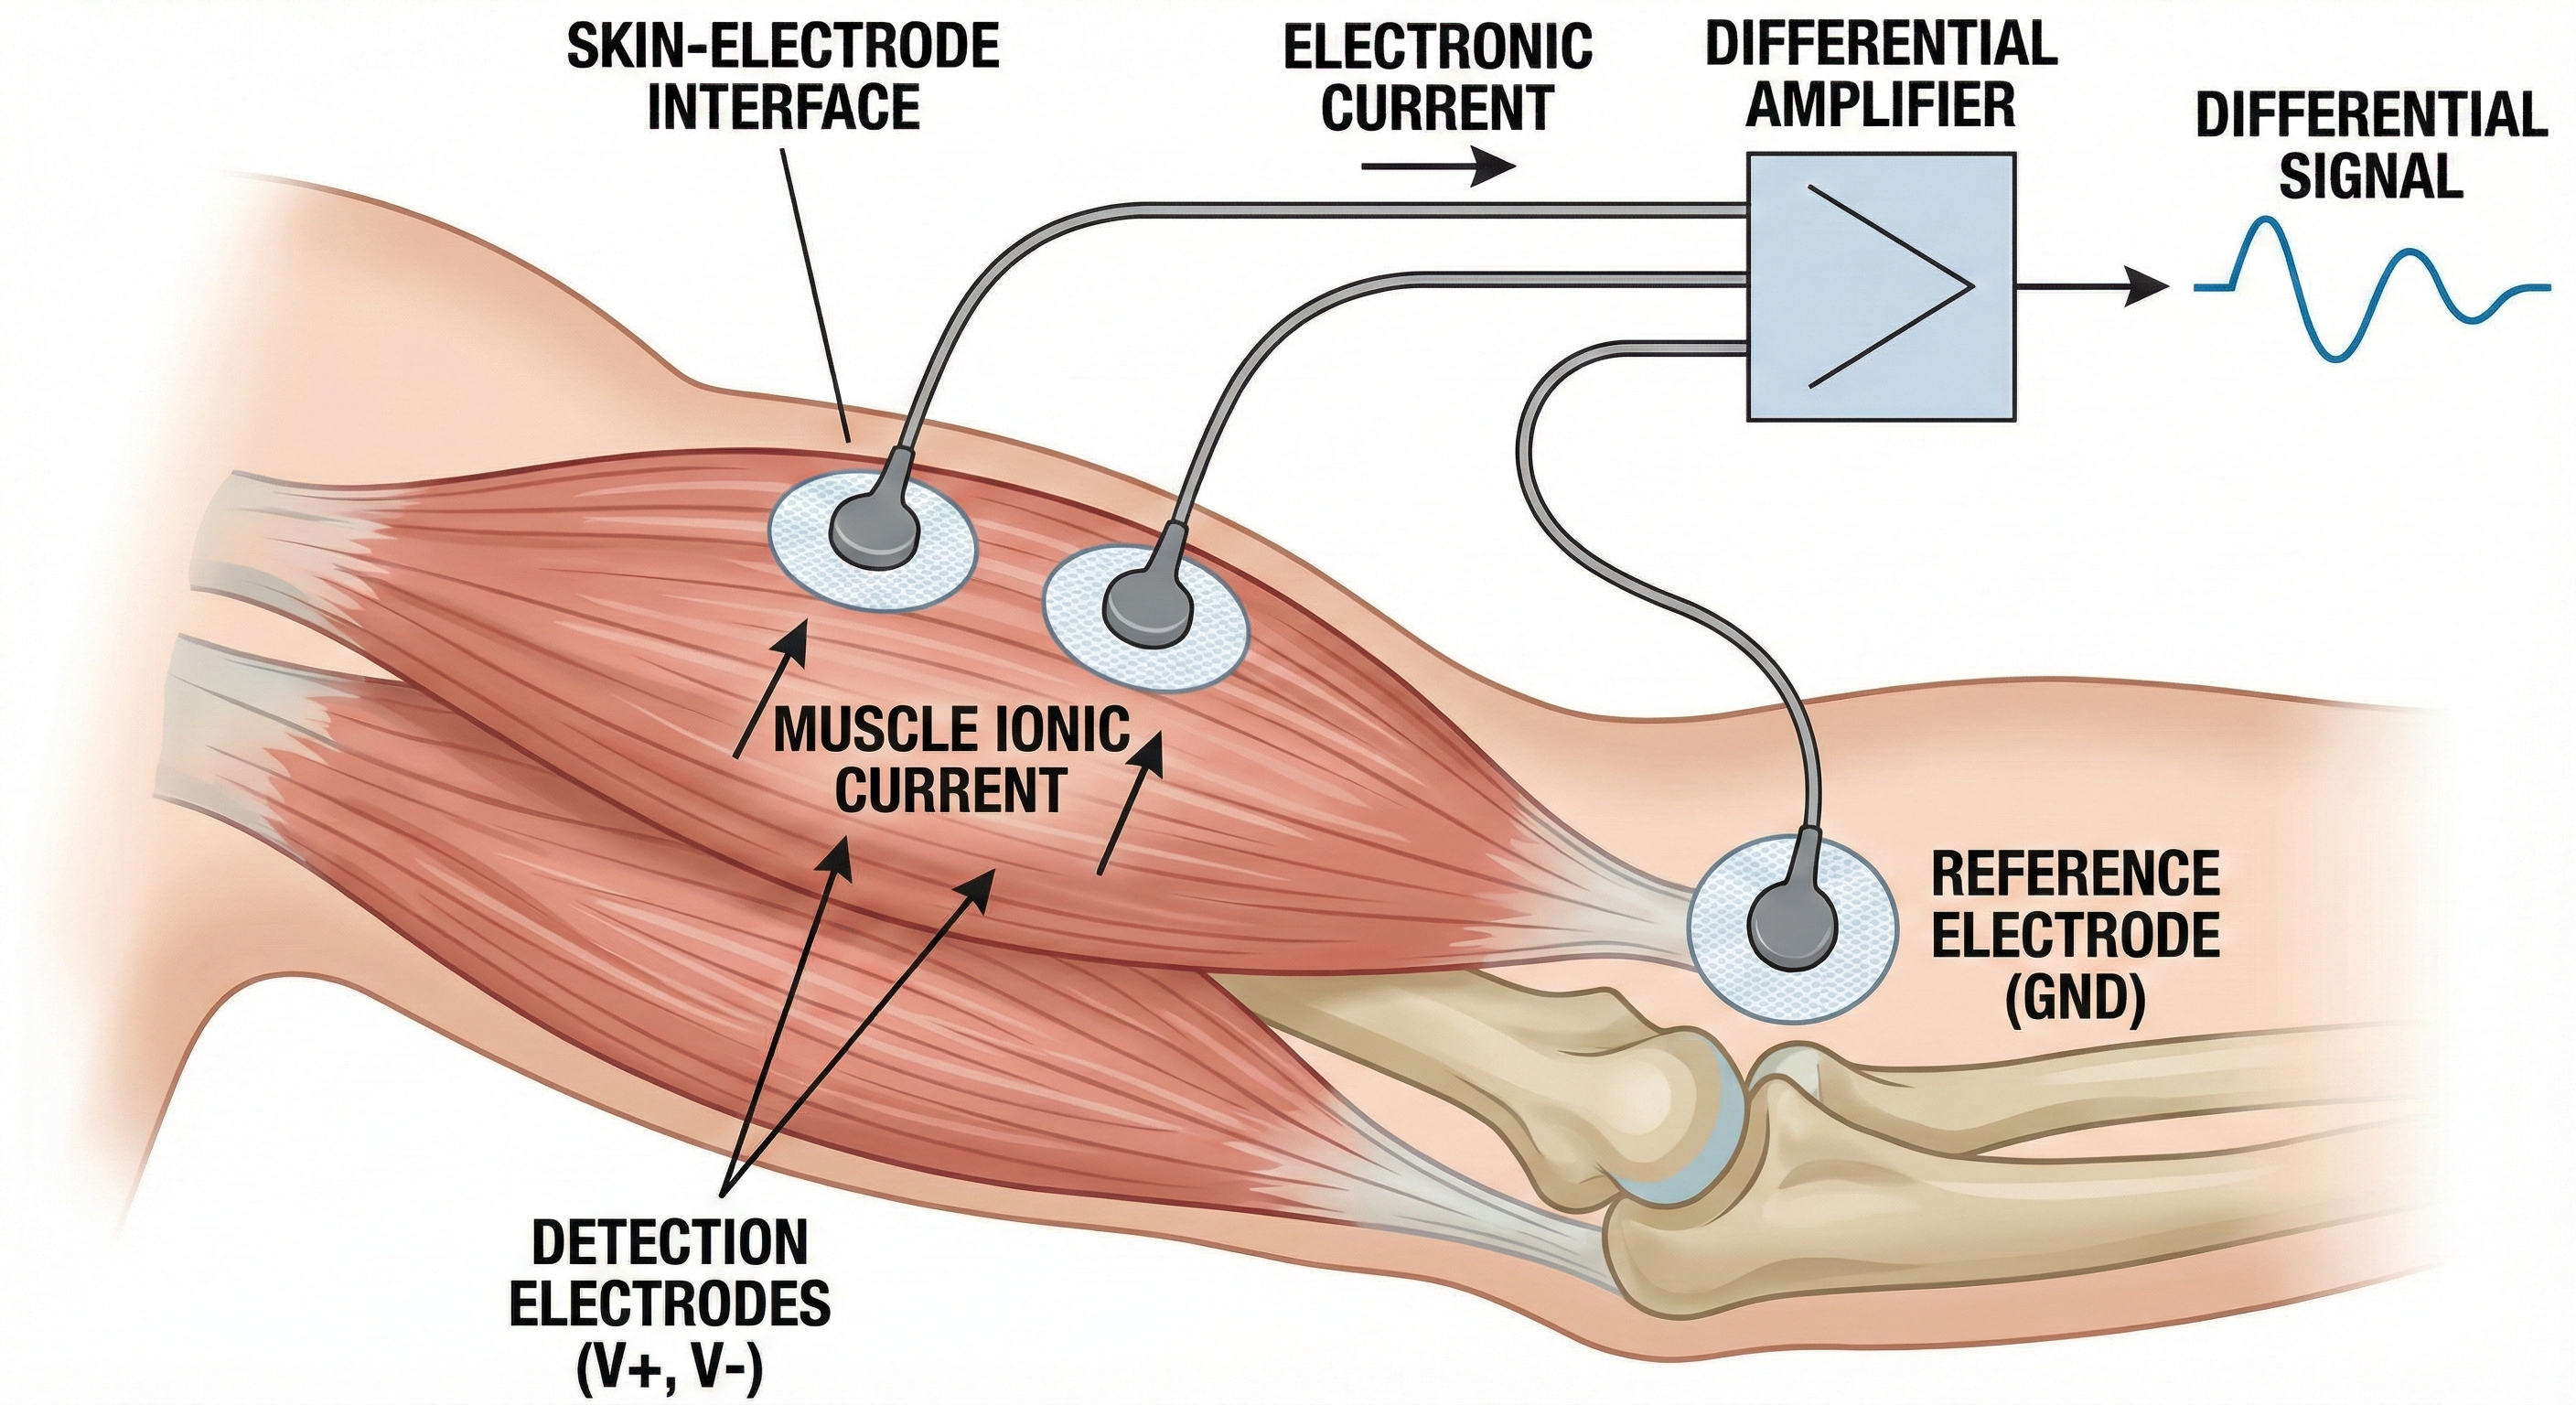
\includegraphics[width=0.8\textwidth]{imagens/eletrodo_illustration.png}
    \caption{Aquisição de biosinais utilizando-se eletrodos de superfícies}
    \label{fig:semg}
\end{figure}

O sinal de EMG bruto é estocástico e apresenta frequências que variam tipicamente entre 10 Hz e 500 Hz, com amplitudes na faixa de microvolts a milivolts \cite{marchetti2006}. Devido a essa natureza complexa, a análise do sinal geralmente requer processamento no domínio do tempo ou da frequência. Uma das técnicas mais comuns para quantificar a intensidade da ativação muscular é o cálculo do valor RMS (Root Mean Square), que reflete a potência do sinal sem a necessidade de retificação prévia, sendo uma métrica robusta para avaliar o nível de atividade elétrica muscular.

\section{Instrumentação e Condicionamento de Sinais}
\label{sec:instrumentacao}

O estágio de instrumentação e condicionamento analógico atua como a ponte entre o fenômeno biológico e o mundo digital. Devido à fragilidade dos biosinais, não é viável conectá-los diretamente a um processador; é necessário um circuito intermediário (\textit{front-end} analógico) capaz de adequar as características elétricas do sinal. As subseções a seguir detalham os três pilares fundamentais desse processo: amplificação, filtragem e conversão analógico-digital.

\subsection{Amplificação de Instrumentação}
A primeira e mais crítica etapa do condicionamento é a amplificação. Como os biopotenciais possuem amplitudes extremamente baixas, muitas vezes imersas em ruído elétrico, o uso de amplificadores operacionais comuns é insuficiente. O principal desafio não é apenas aumentar a amplitude do sinal, mas fazê-lo rejeitando as interferências que atingem o corpo do paciente, que atua como uma antena para o ruído da rede elétrica (60 Hz) e outros ruídos eletromagnéticos causados por equipamentos elétricos.

Para solucionar esse problema, utiliza-se a topologia de Amplificador de Instrumentação (INA). Esse circuito é composto tipicamente por três amplificadores operacionais, conforme ilustrado na Figura \ref{fig:ina}. Diferente de um amplificador comum, o INA possui entradas diferenciais com altíssima impedância, o que evita o carregamento do circuito equivalente da pele.

\begin{figure}[htbp]
  \centering
  \includegraphics[width=0.8\textwidth]{imagens/INA illustration.png}
  \caption{Topologia interna do Amplificador de Instrumentação AD620}
  \label{fig:ina}
  \source{Analog Devices \cite{ad620datasheet}}
\end{figure}

Sua principal figura de mérito é a Taxa de Rejeição de Modo Comum (CMRR - \textit{Common-Mode Rejection Ratio}). O CMRR mede a capacidade do amplificador de rejeitar sinais que aparecem iguais em ambas as entradas (como o ruído de rede induzido no corpo) e amplificar apenas a diferença de potencial entre os eletrodos (o sinal biológico real). Segundo \cite{carr2001}, para aplicações biomédicas de alta fidelidade, é desejável um CMRR superior a 90 dB.

\subsection{Filtragem Analógica Ativa}
Após a amplificação, o sinal ainda pode conter componentes indesejados fora da faixa de interesse fisiológico, como flutuações de linha de base (baixa frequência) causadas pela respiração ou ruídos eletromagnéticos de alta frequência. A filtragem analógica é necessária para limitar a largura de banda do sinal antes da digitalização, melhorando a relação sinal-ruído (SNR) e prevenindo o falseamento de dados (\textit{aliasing}).

Existem diversas topologias de filtros (Bessel, Chebyshev, Butterworth), mas a escolha para bioinstrumentação geralmente recai sobre filtros ativos com resposta Butterworth. Conforme destacam \cite{balbinot2019v1} e \cite{marchetti2006}, o filtro Butterworth é preferido por apresentar uma resposta "maximamente plana" na banda de passagem. Isso significa que ele não introduz oscilações (\textit{ripples}) na amplitude das frequências de interesse, preservando a linearidade e a morfologia das ondas do ECG e EMG, o que é crucial para o diagnóstico clínico preciso.

\subsection{Conversão Analógico-Digital (A/D)}
A etapa final do hardware é a Conversão Analógico-Digital (ADC), que transforma a tensão elétrica contínua em uma sequência discreta de valores binários processáveis por algoritmos computacionais. A qualidade desta conversão é definida principalmente por dois parâmetros: a taxa de amostragem e a resolução.

A taxa de amostragem deve obedecer ao Teorema de Nyquist, sendo pelo menos o dobro da maior frequência contida no sinal para evitar perdas de informação. Já a resolução, medida em bits, define a "granularidade" da medida. Microcontroladores comuns (como o Arduino Uno) tipicamente possuem ADCs de 10 bits, o que divide a faixa de leitura em apenas 1024 níveis. Para aplicações de biosinais de alta precisão, onde micro-variações são diagnósticas, recomenda-se o uso de ADCs externos de maior resolução (como 16 bits ou superior), permitindo detectar nuances do sinal que seriam perdidas em quantizações mais grosseiras \cite{balbinot2019v1}.

\section{Filtragem Digital e Inteligência Artificial}
\label{sec:filtragem_ia}

O tratamento de sinais biomédicos exige técnicas robustas para garantir que a informação fisiológica não seja mascarada por ruídos. Esta seção aborda desde os métodos clássicos de processamento digital até as abordagens modernas baseadas em aprendizado de máquina.

\subsection{Filtragem Digital}

A filtragem digital é o processo matemático realizado sobre um sinal discreto (amostrado) com o objetivo de modificar seu espectro de frequência, atenuando componentes indesejados e preservando a informação relevante. Segundo \cite{balbinot2019v1}, os filtros digitais são classificados fundamentalmente em duas categorias baseadas em sua resposta ao impulso: Filtros de Resposta ao Impulso Finita (FIR) e Filtros de Resposta ao Impulso Infinita (IIR). Os filtros FIR são inerentemente estáveis e possuem fase linear, o que é crucial para evitar distorções na morfologia de sinais como o ECG, embora exijam maior ordem (e custo computacional) para atingir cortes abruptos de frequência.

Já os filtros IIR, conforme explica \cite{balbinot2019v1}, conseguem mimetizar o comportamento de filtros analógicos clássicos (como Butterworth ou Chebyshev) com menor custo computacional e menor atraso de sinal. No entanto, eles podem apresentar instabilidade devido à realimentação e não possuem fase linear perfeita. Embora eficazes para ruídos estacionários (como a interferência de 60 Hz da rede elétrica), técnicas de filtragem digital clássica muitas vezes falham em remover artefatos não-estacionários e complexos, como o ruído de movimento muscular, sem degradar o sinal de interesse, o que motiva a busca por métodos adaptativos baseados em inteligência artificial.

\subsection{Inteligência Artificial (IA)}

A Inteligência Artificial (IA) pode ser definida como a capacidade de uma máquina realizar tarefas que, tradicionalmente, exigiriam inteligência humana. Isso inclui habilidades cognitivas como reconhecimento de padrões, compreensão de linguagem natural, percepção visual e tomada de decisão. O campo da IA é vasto e abrange subáreas como robótica, visão computacional e processamento de linguagem natural, buscando mimetizar a capacidade humana de raciocinar e interagir com o ambiente.

No contexto de biosinais, a IA permite que sistemas computacionais analisem grandes volumes de dados fisiológicos para identificar anomalias ou limpar sinais de forma mais eficiente que algoritmos determinísticos. Uma das vertentes mais promissoras para essa tarefa é o \textit{Deep Learning}, que utiliza estruturas matemáticas inspiradas no cérebro biológico para aprender representações complexas de dados a partir de exemplos, sem a necessidade de regras manuais rígidas.

\subsection{Aprendizado de Máquina (\textit{Machine Learning})}

O Aprendizado de Máquina, ou \textit{Machine Learning} (ML), é a ciência de fazer com que computadores ajam sem serem explicitamente programados para cada situação específica. É um subcampo da IA onde algoritmos analisam dados, aprendem com eles e fazem previsões ou decisões baseadas nos padrões encontrados. Segundo \cite{goodfellow2016}, as dificuldades enfrentadas por sistemas que dependem de conhecimento codificado rigidamente sugerem que os sistemas de IA precisam da capacidade de adquirir seu próprio conhecimento, extraindo padrões de dados brutos. Essa capacidade é conhecida como aprendizado de máquina.

Computadores são historicamente eficientes em tarefas que podem ser formalizadas matematicamente, mas falham em tarefas subjetivas ou intuitivas para humanos, como reconhecer um rosto ou interpretar um sinal ruidoso. O ML resolve isso através de paradigmas de aprendizado, que podem ser: supervisionado (onde o sistema é treinado com pares de entrada-saída rotulados), não supervisionado (onde o sistema busca estruturas ocultas em dados não rotulados) e aprendizado por reforço (baseado em recompensas e punições). Essa capacidade de generalização permite categorizar objetos, prever tendências futuras e, no escopo deste trabalho, distinguir entre o sinal cardíaco real e o ruído de fundo.

\subsection{Redes Neurais Artificiais}

As Redes Neurais Artificiais (RNAs) são modelos computacionais inspirados no funcionamento do sistema nervoso central humano. Elas são compostas por unidades de processamento elementares, chamadas de neurônios artificiais, que são interconectadas através de canais de comunicação associados a valores numéricos conhecidos como "pesos". O princípio básico é que a rede aprende ajustando esses pesos: cada vez que um caminho leva a uma decisão correta durante o treinamento, as conexões envolvidas são fortalecidas matematicamente.

Uma RNA é tipicamente organizada em camadas: uma camada de entrada (que recebe os dados brutos), uma ou mais camadas ocultas (onde ocorre o processamento e extração de características) e uma camada de saída. Cada neurônio processa seus dados de entrada através de uma função de ativação não-linear e transmite o resultado para a próxima camada. Essa arquitetura permite que a rede modele relações complexas e não-lineares entre as entradas e as saídas, sendo ideal para o processamento de sinais biológicos que variam dinamicamente.

\subsection{Aprendizado Profundo (\textit{Deep Learning})}

O \textit{Deep Learning} (Aprendizado Profundo) é uma subárea do \textit{Machine Learning} que se concentra no treinamento de redes neurais com muitas camadas ocultas (daí o termo "profundo"). Segundo \cite{dsa2022}, essa profundidade permite que o algoritmo modele e aprenda representações dos dados em múltiplos níveis de abstração. Enquanto as camadas iniciais podem aprender a detectar pequenas variações locais no sinal, as camadas mais profundas combinam essas informações para reconhecer morfologias complexas, como o complexo QRS de um ECG.

Para viabilizar o \textit{Deep Learning}, é necessário um grande volume de dados para treinamento e um alto poder computacional, frequentemente suprido pelo uso de Unidades de Processamento Gráfico (GPUs), que aceleram as operações matriciais massivas envolvidas no processo. Conforme \cite{goodfellow2016}, o \textit{Deep Learning} resolve o problema central da aprendizagem de representações, permitindo que o computador construa conceitos complexos a partir de conceitos mais simples, superando a performance de algoritmos tradicionais em tarefas de percepção como visão e audição.

\subsection{Redes Neurais Convolucionais (CNNs)}

As Redes Neurais Convolucionais (CNNs) são uma classe especializada de redes neurais profundas, projetadas originalmente para processar dados que possuem uma topologia de grade, como imagens bidimensionais (2D). No entanto, elas têm se mostrado extremamente eficazes para o processamento de séries temporais unidimensionais (1D), como os sinais de ECG e EMG \cite{lomoio2024}. A principal característica das CNNs é o uso da operação matemática de convolução, onde filtros (ou \textit{kernels}) deslizam sobre o sinal de entrada para extrair características locais relevantes, independentemente de sua posição no tempo, conferindo invariância à translação.

Em aplicações de \textit{denoising} (remoção de ruído) de biosinais, as CNNs 1D conseguem aprender a morfologia das ondas características, como a onda R do ECG, e diferenciá-las de ruídos aleatórios \cite{lomoio2024}. A arquitetura típica envolve camadas de convolução para extração de \textit{features}, seguidas por camadas de \textit{pooling} (subamostragem), que reduzem a dimensionalidade e aumentam a robustez do modelo a pequenas variações temporais, permitindo uma filtragem adaptativa que preserva a forma do sinal clínico \cite{goodfellow2016, lomoio2024}.

\subsection{Autoencoders}

Os Autoencoders são um tipo de rede neural utilizada para aprendizado não supervisionado, cujo objetivo principal é aprender uma representação compacta (codificação) dos dados de entrada. A arquitetura de um autoencoder é composta por duas partes principais: o \textit{Encoder}, que comprime a entrada em uma representação de menor dimensão (espaço latente), e o \textit{Decoder}, que tenta reconstruir a entrada original a partir dessa representação comprimida. O aprendizado ocorre minimizando a diferença entre a entrada e a saída reconstruída.

Para a redução de ruído, utiliza-se uma variação conhecida como \textit{Denoising Autoencoder} (DAE). Neste método, o modelo é treinado introduzindo-se propositalmente ruído no sinal de entrada, mas forçando a rede a compará-lo com o sinal limpo na saída. Com isso, o Autoencoder é obrigado a aprender as características estruturais robustas do biosinal (como a periodicidade do ECG) e a ignorar o ruído, pois o ruído é aleatório e não possui padrão passível de compressão eficiente no espaço latente. Isso torna os DAEs ferramentas poderosas para limpar sinais biomédicos degradados \cite{lomoio2024}.
% -------------------------------------------------------------------------
% CAPÍTULO 3: TRABALHOS RELACIONADOS
% -------------------------------------------------------------------------
\chapter{Trabalhos Relacionados}
\label{chap:trabalhos_relacionados}

A aquisição e o processamento de sinais biológicos, devido à sua baixa amplitude e alta suscetibilidade a ruídos, são temas amplamente investigados na literatura científica. Os esforços da comunidade de pesquisa dividem-se historicamente em duas frentes principais: a otimização de circuitos eletrônicos (\textit{hardware}) para melhorar a relação sinal-ruído no momento da captação, e o desenvolvimento de algoritmos avançados (\textit{software}) para a filtragem e reconstrução do sinal digitalizado. Esta seção apresenta as principais contribuições recentes em ambas as áreas, fornecendo o embasamento necessário para a arquitetura proposta neste trabalho.

\section{Avanços em Hardware e Instrumentação Analógica}

No escopo da miniaturização e eficiência energética, \cite{kim2016} propuseram um System on Chip (SoC) reconfigurável focado em plataformas vestíveis (wearables) de baixa potência. O trabalho abordou o desafio de adquirir múltiplos parâmetros fisiológicos com modalidades distintas, incluindo Eletropotencial (como ECG), Bioimpedância, Eletroquímico (glicose) e Fotoelétrico (PPG). Os autores desenvolveram um front-end analógico que pode compartilhar blocos de amplificação e filtragem entre esses diferentes modos de sensoriamento, alcançando um consumo de energia menor que 52 µW por canal. A conclusão central do estudo evidenciou que a integração de hardware analógico reconfigurável reduz a complexidade de fabricação e o tamanho do sistema, ao diminuir a quantidade de chips necessários para aquisições multifuncionais.

Focando na qualidade da captação do sinal em ambientes com interferência, \cite{singh2018} projetaram um Amplificador de Instrumentação (INA) CMOS de baixo ruído e alto ganho. Os autores destacam o desafio de extrair sinais biomédicos fracos, na ordem de poucos milivolts, que possuem níveis de amplitude quase equivalentes aos de ruído. Utilizando uma topologia de três amplificadores operacionais com um estágio de saída do tipo folded cascode , o design alcançou um ganho total de 67,7 dB e uma Taxa de Rejeição de Modo Comum (CMRR) de 92 dB. O estudo concluiu que a arquitetura proposta, consumindo apenas 263 µW, oferece o baixo ruído e o alto ganho necessários para o processamento de sinais biomédicos.

Dando continuidade às pesquisas sobre \textit{front-ends} de precisão, \cite{pathak2025} detalharam o projeto de amplificadores operacionais de baixo ruído voltados especificamente para a instrumentação biomédica. O trabalho concentrou-se no equacionamento do compromisso (\textit{trade-off}) entre ganho, consumo de energia e ruído térmico e de cintilação (\textit{flicker noise}) gerado pelos próprios transistores. A simulação da arquitetura de dois estágios operou com uma potência de 87 $\mu$W, entregando um ganho de 84 dB, um CMRR superior a 100 dB e alcançando um ruído referido à entrada excepcionalmente baixo, na marca de 10 nV/$\sqrt{\text{Hz}}$ (especificamente 9,5 nV/$\sqrt{\text{Hz}}$ a 1 kHz). A conclusão apontou que o dimensionamento geométrico preciso e a escolha da topologia dos componentes analógicos permitem uma redução drástica nesse nível de ruído, validando a importância de utilizar \textit{hardware low-noise} como primeira linha de defesa contra a degradação de biopotenciais.

\section{Evolução da Filtragem: Do Processamento Clássico à Inteligência Artificial}

Embora o hardware desempenhe um papel crucial, a eliminação de ruídos com sobreposição de frequência, como a interferência eletromiográfica (EMG), exige processamento digital avançado. Explorando esse domínio, \cite{wang2019} propuseram um método inovador focado no design de uma nova wavelet para a remoção de ruído em sinais de ECG. Em vez de propor novas regras de limiarização, os autores otimizaram os coeficientes do filtro para aproximar a resposta de um filtro ideal, construindo uma wavelet ortogonal quase simétrica (denominada wavelet fibr). Testado com dados clínicos reais e com sinais simulados de fibrilação atrial, o método obteve maiores valores de Relação Sinal-Ruído (SNR) e menor Erro Quadrático Médio (MSE) frente a wavelets tradicionais como db4 e sym4. A conclusão do estudo evidenciou que a wavelet modificada é altamente eficaz na remoção de ruídos de alta frequência, conseguindo preservar e realçar características fracas do sinal, como as ondas P, T e as ondas F, que normalmente seriam atenuadas no processo de filtragem.

A transição dos métodos matemáticos determinísticos para o Aprendizado de Máquina foi aprofundada por \cite{antczak2018}, que propôs o uso de Redes Neurais Recorrentes Profundas (DRNNs) para o \textit{denoising} de ECG. O estudo abordou a limitação dos filtros convencionais, que tendem a distorcer o sinal clínico quando há sobreposição espectral entre o ruído e a informação biológica. Utilizando uma arquitetura baseada em células LSTM (\textit{Long Short-Term Memory}), o autor introduziu uma estratégia de \textit{Transfer Learning}: a rede foi pré-treinada com dados sintéticos gerados por um modelo dinâmico de ECG para aprender a morfologia ideal do sinal, sendo posteriormente refinada (\textit{fine-tuning}) com dados reais. Os resultados demonstraram que essa abordagem supera métodos de referência, especialmente em cenários com alta contaminação de ruído, evidenciando que modelos de \textit{Deep Learning} podem isolar características fisiológicas complexas sem a necessidade do projeto manual de filtros para cada tipo de interferência.

Elevando a capacidade das redes neurais, \cite{lomoio2024} apresentaram o modelo DCAE-SR, que propõe uma abordagem inovadora: um Autoencoder Convolucional voltado não apenas para a remoção de ruídos (\textit{denoising}), mas também para a reconstrução do sinal em super-resolução. Utilizando Redes Neurais Convolucionais 1D (Conv1D), o modelo extrai recursos espaciais do sinal corrompido e os comprime em um espaço latente. A grande inovação da arquitetura reside no uso de dois decodificadores paralelos: um responsável por reconstruir o sinal na sua resolução original e outro focado exclusivamente em gerar uma onda limpa com uma taxa de amostragem significativamente superior à original (elevando de 50 Hz para 500 Hz). A pesquisa concluiu que os \textit{Autoencoders} são ferramentas formidáveis em instrumentação, pois conseguem recuperar detalhes morfológicos finos (como os complexos P, QRS e a onda T) que normalmente seriam obliterados por equipamentos de aquisição de baixa resolução ou artefatos de ruído.

\section{Diferencial do Trabalho Proposto}

A análise da literatura revela que os projetos frequentemente tratam a instrumentação biomédica de forma isolada: ou focam na construção de microchips altamente específicos e inacessíveis para o público geral (Kim; Ko, 2016; Goel; Singh, 2013; Pathak et al., 2025), ou dependem exclusivamente de processamento digital avançado e complexas redes neurais para limpar sinais que já foram adquiridos com baixa qualidade (Wang; Zhu; Yan; Yang, 2019; Antczak, 2018; Lomoio; Veltri; Guzzi; Liò, 2024).

O presente trabalho se diferencia justamente por propor uma arquitetura holística e integrativa que une o melhor de ambas as abordagens. Em contraste com soluções do tipo \textit{System on Chip} fechadas, propõe-se um \textit{front-end} analógico com componentes discretos de prateleira (utilizando CIs de alto CMRR, baseados nos princípios validados por (Goel; Singh, 2013) e (Pathak et al., 2025)), configurando um \textit{shield} acessível e replicável. Além disso, em vez de depender apenas dessa etapa física, o sistema translada os dados para uma estação de processamento secundária, aplicando o poder dos \textit{Autoencoders} de \textit{Deep Learning} no domínio digital. Essa sinergia garante que a Inteligência Artificial trabalhe não sobre um sinal totalmente corrompido, mas sobre um sinal pré-condicionado, permitindo a extração de métricas de alta fidelidade clínica utilizando plataformas de hardware de baixo custo.

% -------------------------------------------------------------------------
% CAPÍTULO 4: DESENVOLVIMENTO
% -------------------------------------------------------------------------

\chapter{Metodologia e Desenvolvimento}
\label{chap:desenvolvimento}

Este capítulo documenta as etapas técnicas de desenvolvimento do projeto, desde a concepção da arquitetura de \textit{hardware} até a implementação dos algoritmos de \textit{software}. A metodologia segue uma abordagem incremental, iniciando pela validação teórica e simulação, seguida pela prototipagem física e integração dos sistemas.

\section{Definição da Arquitetura do Sistema}

Para o desenvolvimento de sistemas de instrumentação biomédica, a literatura apresenta diferentes abordagens de topologia. Após análise comparativa de viabilidade e desempenho, optou-se pela **Topologia Híbrida (Condicionamento Analógico + Processamento Remoto)**.

Nesta arquitetura, o \textit{hardware} analógico (o \textit{shield} proposto) realiza o condicionamento crítico — amplificação de instrumentação e filtragem de frequências espúrias —, entregando um sinal limpo e com amplitude adequada ao conversor A/D. O processamento digital pesado, incluindo a filtragem avançada por Inteligência Artificial, é delegado a um computador. Esta decisão permite utilizar microcontroladores de baixo custo como interface de comunicação, garantindo ao mesmo tempo que o sinal digitalizado possua qualidade suficiente para análise.

\subsection{Detalhamento dos Blocos Funcionais}

A arquitetura foi dividida em quatro macro-blocos funcionais:

\begin{enumerate}
    \item \textbf{Bloco de Aquisição Analógica (\textit{Front-End}):} Responsável pela interface com o paciente. Utiliza um Amplificador de Instrumentação (INA) para garantir alta Razão de Rejeição em Modo Comum (CMRR) e estágios de filtragem ativa (Passa-Alta e Passa-Baixa) para delimitar a banda de frequência dos biosinais.
    
    \item \textbf{Bloco de Conversão e Controle:} Composto pelo microcontrolador e um Conversor Analógico-Digital (ADC) externo de 16-bits. O uso de um ADC externo visa superar as limitações de resolução dos conversores nativos (geralmente 10-bits), permitindo a detecção de micro-variações no sinal.
    
    \item \textbf{Bloco de Comunicação:} Interface (USB/Serial) responsável pelo transporte do fluxo de dados digitais do \textit{hardware} para a estação de trabalho em tempo real.
    
    \item \textbf{Bloco de Processamento Inteligente (Software):} Executado em computador, este módulo recebe os dados brutos, realiza o pré-processamento digital e aplica o modelo de Inteligência Artificial para a remoção final de artefatos complexos e visualização gráfica.
\end{enumerate}

\section{Projeto do Hardware de Aquisição}

Esta seção detalha a seleção de componentes e o dimensionamento dos circuitos analógicos.

\subsection{Seleção de Componentes Críticos}

A escolha dos componentes priorizou especificações de baixo ruído e alta fidelidade. A Tabela \ref{tab:componentes} resume a seleção final.

\begin{table}[H]
\centering
\caption{Definição dos Componentes Críticos do Hardware}
\label{tab:componentes}
\begin{tabular}{p{4cm} p{3cm} p{7cm}}
\toprule
\textbf{Função} & \textbf{Componente} & \textbf{Justificativa Técnica} \\
\midrule
Amplificação de Instrumentação & AD620 & Padrão médico devido ao alto CMRR ($>100$ dB) e ganho ajustável com um único resistor. \\
\midrule
Filtragem Ativa (Op-Amps) & OPA2134 & Baixíssima distorção e ruído, ideal para bioinstrumentação de alta fidelidade. \\
\midrule
Conversão A/D (ADC) & ADS1115 & Resolução de 16-bits e interface I2C, superior aos ADCs nativos de microcontroladores comuns. \\
\midrule
Microcontrolador & Arduino Uno R3 & Plataforma acessível para controle do ADC e interface serial com o PC. \\
\midrule
Isolação de Energia & B0505S-1W & Conversor DC-DC para isolar a alimentação do circuito analógico, reduzindo ruído da fonte USB. \\
\bottomrule
\end{tabular}
\end{table}

\subsection{Dimensionamento dos Filtros Analógicos}
% [INSERIR OS CÁLCULOS DOS RESISTORES/CAPACITORES FUTURAMENTE]
O condicionamento analógico inclui filtros ativos de segunda ordem configurados para uma banda passante entre 0,5 Hz e 100 Hz (para ECG) e até 500 Hz (para EMG), visando eliminar componentes DC e ruídos de alta frequência antes da digitalização.

\section{Desenvolvimento do Software e Interface}

Paralelamente ao desenvolvimento do hardware, foi implementado o software base para aquisição e visualização dos dados.

\subsection{Ambiente de Simulação e Validação}

Para validar a lógica de processamento e a interface gráfica antes da finalização do protótipo físico, desenvolveu-se um módulo de simulação em linguagem Python. Este software utiliza dados reais do banco de dados \textit{MIT-BIH Arrhythmia Database} (PhysioNet), reconhecido mundialmente como padrão para validação de algoritmos de ECG.

Utilizou-se o registro ``100'' do banco de dados, contendo sinais digitalizados a 360 Hz. O software emula o comportamento do microcontrolador, lendo os dados brutos (\texttt{.dat}) e enviando-os para a rotina de plotagem como se estivessem sendo adquiridos em tempo real. Isso permite testar a estabilidade da taxa de atualização da interface e a visualização da morfologia do complexo QRS (utilizando a derivação MLII do registro).

\subsection{Interface de Visualização em Tempo Real}

Foi desenvolvida uma interface gráfica utilizando a biblioteca \textit{Matplotlib}. Para garantir fluidez na plotagem de sinais em alta frequência, utilizou-se a técnica de \textit{blitting}, que redesenha apenas os pixels modificados do gráfico a cada quadro de animação. A interface simula um monitor cardíaco, com varredura contínua no domínio do tempo e controles interativos para pausar a aquisição e salvar capturas de tela para análise posterior.

\begin{figure}[htbp]
  \centering
  \includegraphics[width=0.8\textwidth]{imagens/interface_ecg.png}
  \caption{Interface de aquisição de ECG.}
  \label{fig:intecg}
\end{figure}

\section{Processamento Digital e Inteligência Artificial}
% [AQUI ENTRARÁ O CONTEÚDO SOBRE OS FILTROS DIGITAIS QUE AINDA VOU FAZER]
Esta etapa descreverá a implementação dos filtros digitais (FIR/IIR) para remoção de ruído de 60 Hz e o modelo de Rede Neural (Autoencoder) para limpeza avançada do sinal.

\subsection{Filtragem Digital da Interferência de Rede (60 Hz)}

A aquisição de biopotenciais de baixa amplitude, como o ECG, é inerentemente suscetível a interferências eletromagnéticas externas. A fonte de ruído mais ubíqua em ambientes não blindados é a rede elétrica de distribuição, que no Brasil opera na frequência fundamental de 60 Hz. Esse ruído acopla-se capacitivamente aos cabos dos eletrodos e ao corpo do paciente, podendo apresentar amplitudes superiores ao próprio sinal fisiológico de interesse, mascarando ondas cruciais como a onda P e o segmento ST \cite{carr2001}.

Embora o amplificador de instrumentação (hardware analógico) ofereça uma alta Taxa de Rejeição de Modo Comum (CMRR) para atenuar esse ruído na entrada, uma componente residual de 60 Hz frequentemente persiste no sinal digitalizado. Para mitigar esse problema sem distorcer a morfologia do complexo QRS, foi implementada uma etapa de filtragem digital seletiva.

O filtro escolhido para esta aplicação foi um filtro do tipo Notch (rejeita-faixa ou "filtro entalhe") com Resposta ao Impulso Infinita (IIR - Infinite Impulse Response). Filtros IIR são eficientes computacionalmente e conseguem mimetizar o comportamento de filtros analógicos com poucos coeficientes. O filtro Notch é projetado para atenuar severamente uma frequência central específica ($f_0$) e permitir a passagem de todas as outras frequências do espectro \cite{balbinot2019v1}. 

O projeto do filtro foi realizado digitalmente, definindo a frequência central $f_0 = 60 \text{ Hz}$ e um Fator de Qualidade ($Q$). O fator $Q$ determina a seletividade do filtro: um valor alto de $Q$ resulta em uma banda de rejeição extremamente estreita, garantindo que apenas a frequência de 60 Hz seja removida, preservando componentes de frequência adjacentes que são vitais para a integridade do sinal de ECG (como as componentes de alta frequência do complexo QRS). No sistema desenvolvido, utilizou-se um $Q \geq 30$.

Para a aplicação em tempo real, onde o sinal é processado continuamente à medida que é amostrado, a implementação do filtro IIR requer a manutenção do estado interno do filtro (memória das amostras anteriores). A cada nova amostra recebida do conversor A/D, o algoritmo aplica a equação de diferenças do filtro utilizando os coeficientes calculados e o estado anterior das memórias, gerando a amostra filtrada e atualizando o estado para a próxima iteração.

A Figura \ref{fig:filtro_ecg_60hz} demonstra a eficácia desta etapa de processamento. O gráfico superior (A) apresenta um sinal de ECG real (proveniente da base de dados MIT-BIH) contaminado sinteticamente com ruído de 60 Hz, simulando uma condição de aquisição ruidosa. O gráfico inferior (B) exibe o resultado após a passagem pelo filtro Notch digital implementado no firmware do sistema, evidenciando a recuperação da linha de base e a clareza das ondas P, QRS e T.

\begin{figure}[htbp]
  \centering
  \includegraphics[width=0.8\textwidth]{imagens/filtro_60hz.png}
  \caption{Comparativo de Filtragem Digital. A) Sinal de entrada contaminado por ruído de rede de 60 Hz. B) Sinal de saída após aplicação do filtro IIR Notch em tempo real, recuperando a morfologia do ECG.}
  \label{fig:filtro_ecg_60hz}
\end{figure}

\section{Integração e Testes do Sistema}
% [AQUI ENTRARÁ A MONTAGEM FINAL]
Descrição da integração entre o \textit{shield} analógico, o conversor digital e o software de processamento.

% RESULTADOS
\chapter{Resultados}

% CONCLUSÃO
\chapter{Conclusão}

% Bibliografia
\bibliographystyle{abnt}
\bibliography{bibliografia} 

\end{document}